%location/filename: tex/ch1.tex
%author: Anders Østevik
%Last edited: 16.12.2015
%#######--Chapter 3--#######
%Content:
%	Interface/Communication between PC and FPGA
%	

\documentclass[main.tex]{subfiles}

\begin{document}

\chapter{Interface between PC and \acrshort{cru}}

In order for the user to have any control over the \gls{cru}, some sort of serial communication between the users PC and the \gls{fpga} is needed. For now, the communication link is only supposed to monitor and set control signals from the \gls{gbt} bank, and not gather the incoming data. Because of this, speed requirements are not critical. 

A variety of communication protocols were considered and are summed up in the table below. 

Common to all communication systems considered is that they are all duplex systems, which simply means two connected devices that can both transmit and receive signals. While \textit{full-duplex} enables both devices to transmit and receive simoultaneously (telephones), \textit{half-duplex} only enables one device to transmit at a time (walkie-talkies). Common to both is that they have two communication channels. 




\section{Theory of design}


\subsection{Transmission protocol: \gls{rs232}}

Example of an \gls{rs232} setting: 115200-8-N-1

A typical \gls{rs232} datapacket consists of a start bit, followed by 5, 7 or 8 data bits, 1 parity bit and 1 or 2 stop bits. The start bit is typically a logical low and the stop bit(s) high, but this is system dependent. The transmission line remains high until the start bit pulls it down low, and the data transfer begins until the stop bit is reached. The line is then kept high until a new start bit pull it low again for a new data transfer. The figure below shows a typical \gls{rs232} signal.

\begin{figure}[!h]
\begin{center}
\begin{tikzpicture}

\timing [
yscale=2.0,
timing/wscale=3.0,
timing/inline 
node/.style={below left, font=\sffamily\scriptsize}
] at (0,0)
{
H N {$Idle$}
L N {$Start$} 
D {$D_0$} 
D {$D_1$} 
D {$D_2$} 
D {$D_3$} 
D {$D_4$} 
D {$D_5$} 
D {$D_6$}  
D {$D_7$} 
D {$Parity$} 
H N{$Stop$}
%L H N[xscale=.8]{ACK} 
H N{$Idle$}
};

\end{tikzpicture}

\caption{Example of an \gls{rs232} serial signal with 8 data bits, 1 parity bit (ODD or EVEN) and 1 stop bit.}
\label{fig:rs232}

\end{center}
\end{figure}





\subsection{\acrshort{hdl} on the \gls{fpga} side}

Simply put, the \gls{uart} is a circuit that transmits and receives parallel data through a serial line. \cite{chu08}

The \gls{uart}-design is divided into five parts:\\
- A Receiver that receives serial data\\
- A Transmitter that sends serial data.\\
- A Baud Rate Generator that generates the right amount of ticks relative to the baud rate and global clock.\\
- \Gls{fifo}-registers on both the \gls{uart} output and input\\

The following sections gives a brief description of each of the parts described above. \\
The information was parlty obtained by reading chapter 7 from the book \textit{FPGA Prototyping By VHDL Examples} by Pong P. Chu \cite{chu08}, and by studying the \textit{Uart2Bus} \acrshort{vhdl}-design by Arild Velure.

\subsubsection{Oversampling and the Baud Rate Generator}

To obtain an accurate sampling of the received signal, an asynchronous system like the \gls{uart} uses what is referred to as oversampling. \\
With a typical rate of 16 times the baud rate, the receiver listens for the line to go from idle to the first start bit, or from a logical high to a logical low. When low, a counter starts counting from 0 to 7. When the counter reaches 7, the received signal should be in the middle of the start bit. The counter then clears to 0 and starts counting from 0 to 15. This time, when the counter reaches 15, the received signal should be in the middle of the first data bit, or \acrshort{lsb}. The value is retrieved, and the latter procedure is repeated $N - 1$ times until the \acrshort{msb} is retrieved.
If there is a parity bit, the same procedure is repeated one more time to retrieve it. After retrieving all the data bits, the same procedure is used to sample the M stop bits at the end of the signal. After this, the line is held high until a new start bit arrives. 

%\mdfdefinestyle{mystyle}{rightmargin=90pt, linecolor=darkgray}

\begin{figure}[!htp]
\begin{center}
%\begin{minipage}[!h]{0.85\linewidth}  %Needed this to lign the figures up properly
%\begin{mdframed}%[style=mystyle]
\begin{tikztimingtable}[%
    timing/dslope=0.5,
    timing/.style={x=1ex,y=4ex},
    x=4ex,
    timing/rowdist=5ex,
    %timing/coldist=2ex,
    xscale=0.8,yscale=0.7, % scale diagrams
    timing/name/.style={font=\sffamily\scriptsize}
    ]
\\
Data      & 14h 28l 28d{$d_0$} 28d{$d_1$} 28d{$d_2$} \\%16d{$d_3$} 16d{$d_4$} 16d{$d_5$} 16d{$d_6$} 16d{$d_7$} 16d{$stop$}H \\
Sample ticks        & h 125{c}\\
\\
%\vspace{20pt}
%AD   & 2u 1D{addr} 1U{} 1D{$d_1$} D{$d_1 '$} D{$d_2$} 2D{$d_3$} U \\
%C/BE & 2u 1D{0010} 6D{BE\#} U  \\
%IRDY      & UU 4L HLH \\
%TRDY       & UU HLH 3L H \\
%DEVSEL     & 2U 6L H\\
\extracode
\begin{pgfonlayer}{background}
\begin{scope}[semithick]
\vertlines[darkgray, dotted]{1.75, 3.5}
\vertlines[darkgray,dotted]{7.0, 10.5,...,14}
  
  \draw[<->] (1.75,-10) -- (3.5,-10) node [midway,below] {\scriptsize 8 cycles};
  \draw[<->] (3.5,-10) -- (7.0,-10) node [midway,below] {\scriptsize 16 cycles};
    \draw[<->] (7.0,-10) -- (10.5,-10) node [midway,below] {\scriptsize 16 cycles};
      \draw[<->] (10.5,-10) -- (14.0,-10) node [midway,below] {\scriptsize 16 cycles};

  \draw[<-] (3.5, 1) -- (3.5,2) node [midway,above] {\scriptsize Middle};
 \draw[] (3.5, -2.6) -- (3.5,-2.6) node [midway,above] {\tiny Start bit};
  \draw[<-] (7, 1) -- (7,2) node [midway,above] {\scriptsize Sample LSB};
  \draw[<-] (10.5, 1) -- (10.5,2) node [midway,above] {\scriptsize Sample d1};
  \draw[<-] (14, 1) -- (14,2) node [midway,above] {\scriptsize Sample d2};

\end{scope}
\end{pgfonlayer}
\end{tikztimingtable}
%\end{mdframed}
\caption{\gls{uart} receive synchronisation and data sampling points with 16 times the sampling rate.}
\label{fig:uartsample}
%\end{minipage}
\end{center}

\end{figure}


To achieve a sample tick of 16 times the baud rate, a Baud Rate Generator module is implemented into the design. The module generates a one-clock-cycle tick once every $\frac{clock}{16 \times baud\ rate}$ clock cycles. For a baud rate of $115200\ \bit\per\second$ and a clock of $50\ \mega\hertz$, there must be a one-clock-cycle tick once every $27$ clock cycle. This is achieved by counting in certain steps given by the formula below:

\begin{equation}
Baud\ frequency = \frac{16 \times baud\ rate}{GCD(clock, 16 \times baud\ rate)}
\end{equation}

, where GCD is the greatest common divisor between the global clock and the baud rate times 16. \cite{velure10} \\
For a baud rate of $115200\ \bit\per\second$ and a clock of $50\ \mega\hertz$, the counter must count in steps of $576$ per clock cycle. 

Once the counter reaches a given baud limit, the counter resets and the tick-signal is pulled high. After one clock cycle the tick-signal is pulled low again and the counter starts counting. The baud limit is given by:

\begin{equation}
Baud\ limit= \frac{clock}{GCD(clock, 16 \times baud\ rate)} - baud frequency
\end{equation}

, where clock is the global clock of the system and GCD is the greatest common divisor between the global clock and the baud rate times 16. \cite{velure10} \\
For a baud rate of $115200\ \bit\per\second$ and a clock of $50\ \mega\hertz$, the counter must count in steps of $576$ up to the baud limit of $15049$, before resetting and pulling the tick-signal high. 





\end{document}